\documentclass[./answersheet.tex]{subfiles}

\begin{document}
\problem{13}
\begin{wts}
    Explain the TCP Tahoe congestion control procedure. Plot TCP Tahoe \verb|ss_thresh=+oo| and timeout at \verb|rtt3|, plot \verb|rtt=0-9|
\end{wts}
\begin{proof}
    TCP Tahoe does not distinguish between a timeout and 3 duplicate ACKS, and restarts  \verb|cwnd| to \verb|cwnd_init| on either. This is more punishing than TCP Reno. During the initial phase, both TCP flavours start in Slow Start with an unbounded \verb|ss_thresh|, and both \verb|cwnd| exponentially increase per RTT.\\
    
    Once the first timeout is detected, \verb|ss_thresh| is set to half of the timeout \verb|cwnd|, and resumes in slow start. This is required, because TCP is a self-clocking protocol. Since a timeout of the virtual connection indicates that the 'clock' is broken, while duplicate \verb|ACK|s indicate a skipped 'beat' on the clock, but the clocks are still in sync (once in AIMD).\\
    
    The plot is below.\\
    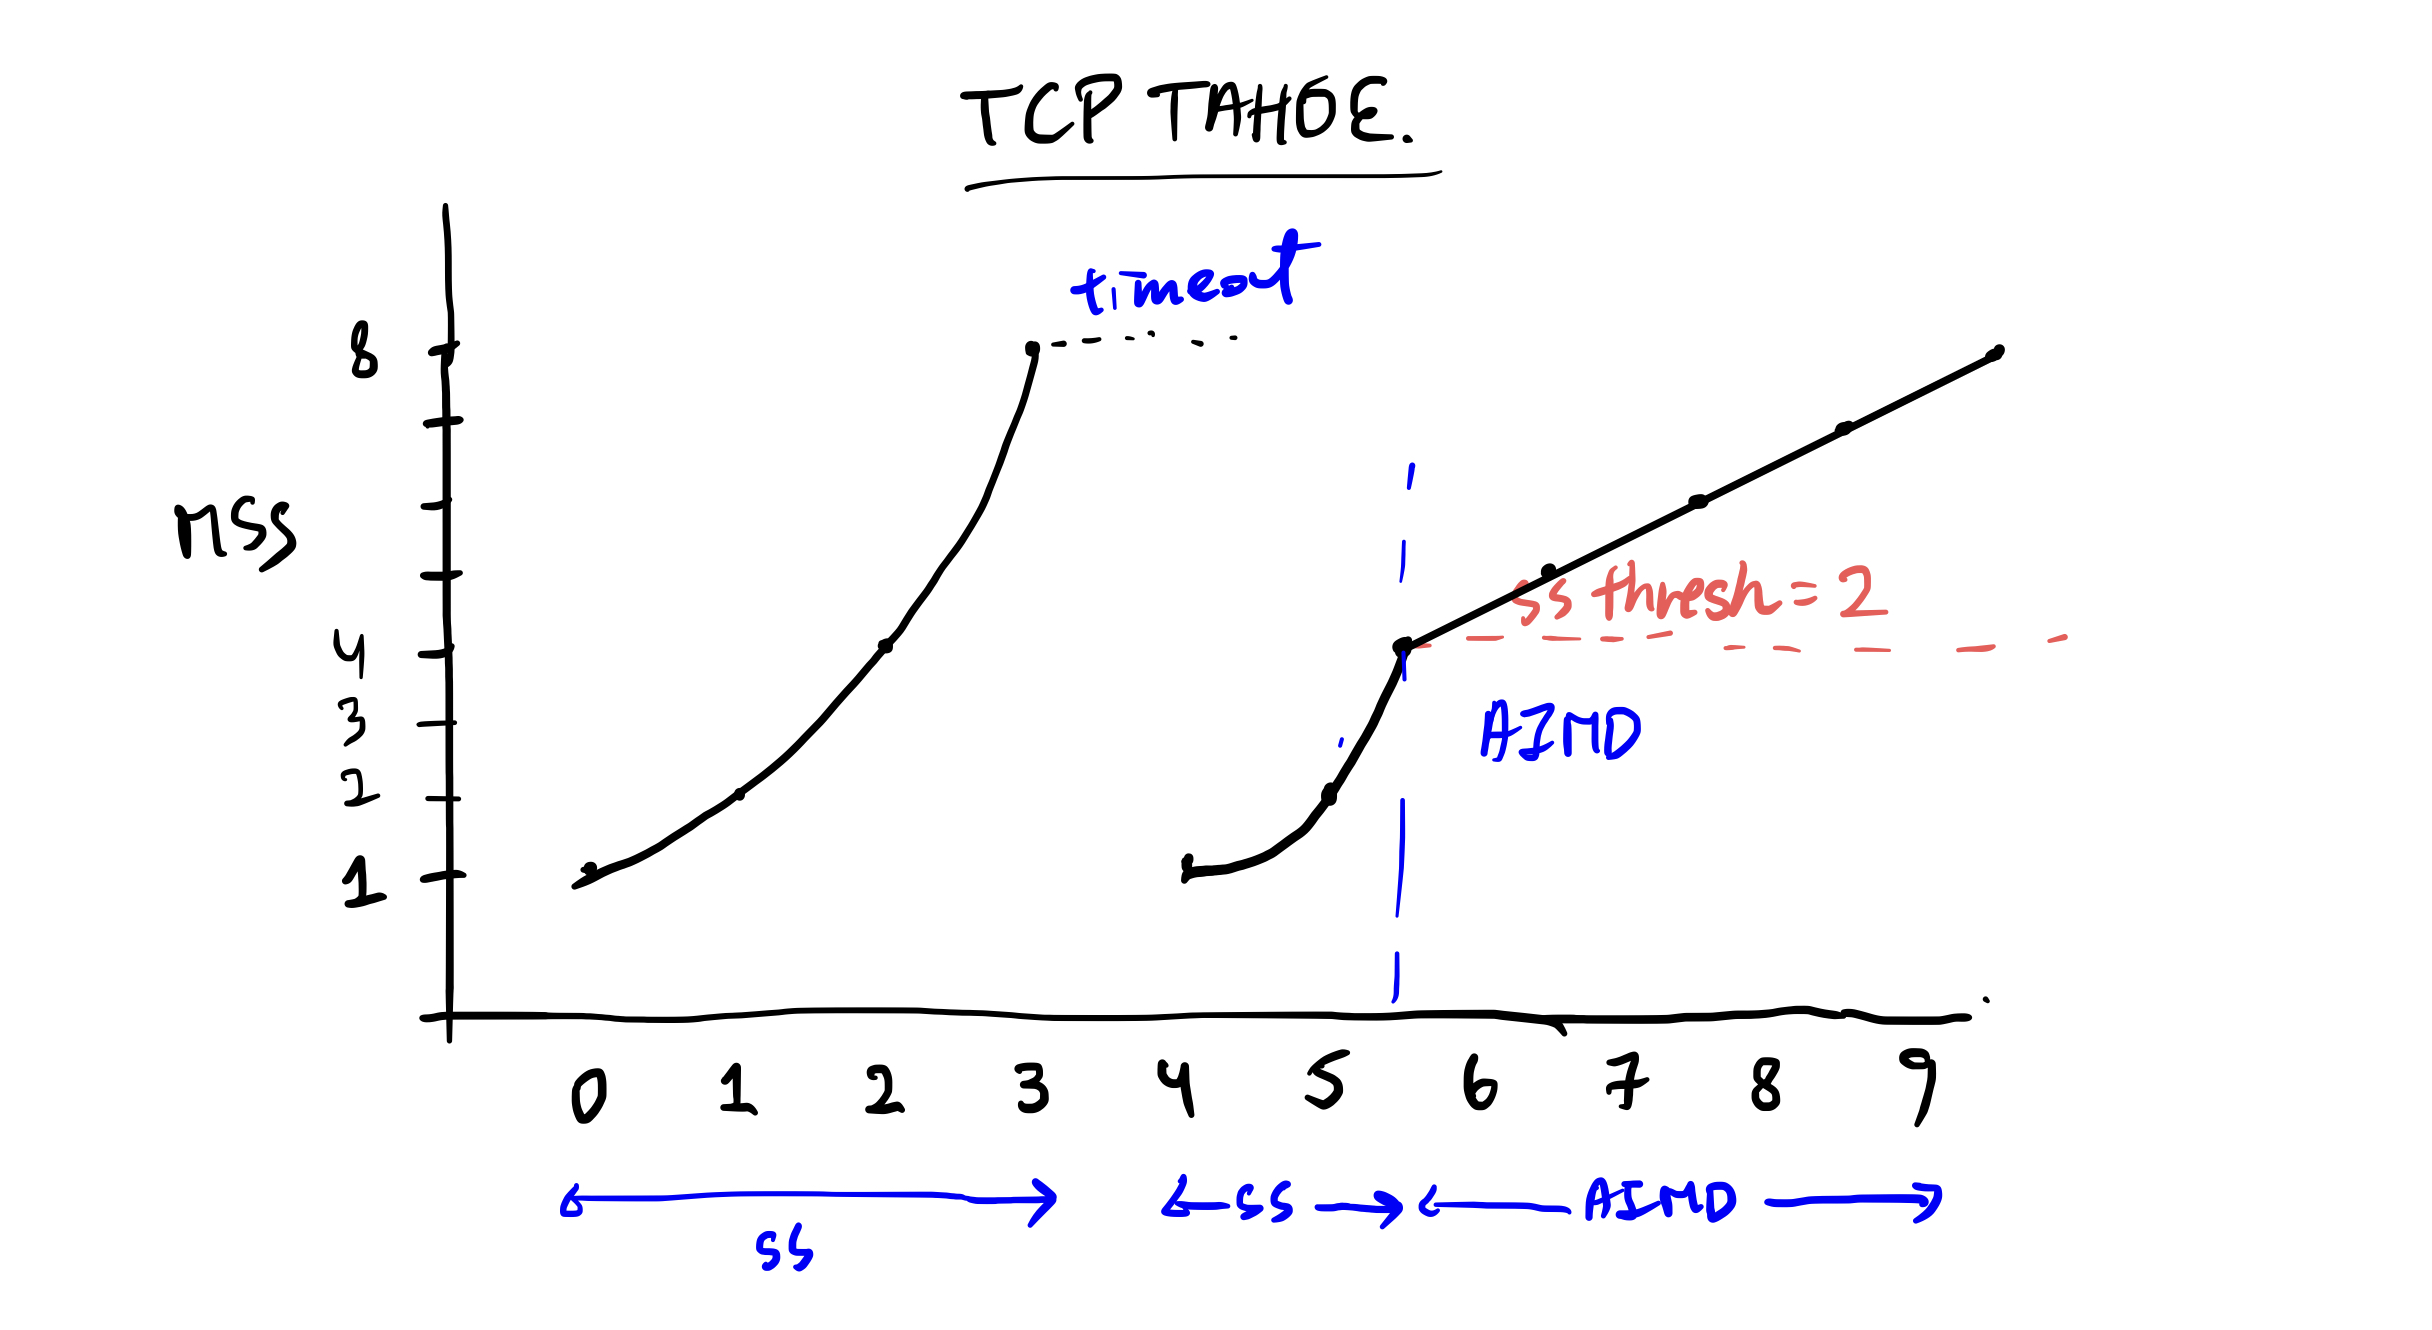
\includegraphics[width=\columnwidth]{./TCP_Q13.jpeg}
    

\end{proof}

\end{document}